% Options for packages loaded elsewhere
\PassOptionsToPackage{unicode}{hyperref}
\PassOptionsToPackage{hyphens}{url}
%
\documentclass[
  letterpaper,
  ignorenonframetext,
  aspectratio=43,
  handout,
  12pt]{beamer}
\usepackage{pgfpages}
\setbeamertemplate{caption}[numbered]
\setbeamertemplate{caption label separator}{: }
\setbeamercolor{caption name}{fg=normal text.fg}
\beamertemplatenavigationsymbolsempty
% Prevent slide breaks in the middle of a paragraph
\widowpenalties 1 10000
\raggedbottom
\setbeamertemplate{part page}{
  \centering
  \begin{beamercolorbox}[sep=16pt,center]{part title}
    \usebeamerfont{part title}\insertpart\par
  \end{beamercolorbox}
}
\setbeamertemplate{section page}{
  \centering
  \begin{beamercolorbox}[sep=12pt,center]{part title}
    \usebeamerfont{section title}\insertsection\par
  \end{beamercolorbox}
}
\setbeamertemplate{subsection page}{
  \centering
  \begin{beamercolorbox}[sep=8pt,center]{part title}
    \usebeamerfont{subsection title}\insertsubsection\par
  \end{beamercolorbox}
}
\AtBeginPart{
  \frame{\partpage}
}
\AtBeginSection{
  \ifbibliography
  \else
    \frame{\sectionpage}
  \fi
}
\AtBeginSubsection{
  \frame{\subsectionpage}
}
\usepackage{amsmath,amssymb}
\usepackage{lmodern}
\usepackage{iftex}
\ifPDFTeX
  \usepackage[T1]{fontenc}
  \usepackage[utf8]{inputenc}
  \usepackage{textcomp} % provide euro and other symbols
\else % if luatex or xetex
  \usepackage{unicode-math}
  \defaultfontfeatures{Scale=MatchLowercase}
  \defaultfontfeatures[\rmfamily]{Ligatures=TeX,Scale=1}
\fi
\usetheme[]{metropolis}
% Use upquote if available, for straight quotes in verbatim environments
\IfFileExists{upquote.sty}{\usepackage{upquote}}{}
\IfFileExists{microtype.sty}{% use microtype if available
  \usepackage[]{microtype}
  \UseMicrotypeSet[protrusion]{basicmath} % disable protrusion for tt fonts
}{}
\makeatletter
\@ifundefined{KOMAClassName}{% if non-KOMA class
  \IfFileExists{parskip.sty}{%
    \usepackage{parskip}
  }{% else
    \setlength{\parindent}{0pt}
    \setlength{\parskip}{6pt plus 2pt minus 1pt}}
}{% if KOMA class
  \KOMAoptions{parskip=half}}
\makeatother
\usepackage{xcolor}
\IfFileExists{xurl.sty}{\usepackage{xurl}}{} % add URL line breaks if available
\IfFileExists{bookmark.sty}{\usepackage{bookmark}}{\usepackage{hyperref}}
\hypersetup{
  hidelinks,
  pdfcreator={LaTeX via pandoc}}
\urlstyle{same} % disable monospaced font for URLs
\newif\ifbibliography
\usepackage{longtable,booktabs,array}
\usepackage{calc} % for calculating minipage widths
\usepackage{caption}
% Make caption package work with longtable
\makeatletter
\def\fnum@table{\tablename~\thetable}
\makeatother
\usepackage{graphicx}
\makeatletter
\def\maxwidth{\ifdim\Gin@nat@width>\linewidth\linewidth\else\Gin@nat@width\fi}
\def\maxheight{\ifdim\Gin@nat@height>\textheight\textheight\else\Gin@nat@height\fi}
\makeatother
% Scale images if necessary, so that they will not overflow the page
% margins by default, and it is still possible to overwrite the defaults
% using explicit options in \includegraphics[width, height, ...]{}
\setkeys{Gin}{width=\maxwidth,height=\maxheight,keepaspectratio}
% Set default figure placement to htbp
\makeatletter
\def\fps@figure{htbp}
\makeatother
% Make links footnotes instead of hotlinks:
\DeclareRobustCommand{\href}[2]{#2\footnote{\url{#1}}}
\setlength{\emergencystretch}{3em} % prevent overfull lines
\providecommand{\tightlist}{%
  \setlength{\itemsep}{0pt}\setlength{\parskip}{0pt}}
\setcounter{secnumdepth}{-\maxdimen} % remove section numbering
\usepackage{pgfpages}
\pgfpagesuselayout{2 on 1}
\providecommand{\tightlist}{%
\setlength{\itemsep}{0pt}\setlength{\parskip}{0pt}}
\makeatletter
\makeatother
\let\Oldincludegraphics\includegraphics
\renewcommand{\includegraphics}[2][]{\Oldincludegraphics[width=\textwidth,height=0.7\textheight,keepaspectratio]{#2}}
\ifLuaTeX
  \usepackage{selnolig}  % disable illegal ligatures
\fi

\author{}
\date{}

\begin{document}

\begin{frame}
Lecture 4 - Eshelby

Dr.~Nicholas Smith

Wichita State University, Department of Aerospace Engineering

27 January 2022
\end{frame}

\begin{frame}{schedule}
\protect\hypertarget{schedule}{}
\begin{itemize}
\tightlist
\item
  27 Jan - 1D Micromechanics (HW1 Due)
\item
  1 Feb - Mean-field
\item
  3 Feb - Orientation Averaging (HW2 Due)
\item
  8 Feb - Variational Calculus
\end{itemize}
\end{frame}

\begin{frame}{outline}
\protect\hypertarget{outline}{}
\begin{itemize}
\tightlist
\item
  eshelby
\item
  aspect ratio
\end{itemize}
\end{frame}

\hypertarget{eshelbys-equivalent-inclusion}{%
\section{eshelby's equivalent
inclusion}\label{eshelbys-equivalent-inclusion}}

\begin{frame}{eshelby}
\protect\hypertarget{eshelby}{}
\begin{itemize}
\tightlist
\item
  Eshelby formulated the exact elastic solution for an elliptical
  inclusion in an infinite matrix
\item
  While this is not often useful, it serves as an exact analytical model
  to compare numerical results with
\item
  It is also the base for more useful mean-field theories
\end{itemize}
\end{frame}

\begin{frame}{eshelby's thought experiment}
\protect\hypertarget{eshelbys-thought-experiment}{}
\begin{itemize}
\tightlist
\item
  Eshelby solution starts with a thought experiment
\item
  Suppose we have a homogeneous, elastic body in equilibrium
\item
  We now cut an ellipsoidal pieces out of that body and allow it to
  undergo a stress-free transformation, such as thermal expansion
\item
  This stress-free transformation is referred to as the transformation
  strain, \(\epsilon^T\)
\end{itemize}
\end{frame}

\begin{frame}{eshelby's thought experiment}
\protect\hypertarget{eshelbys-thought-experiment-1}{}
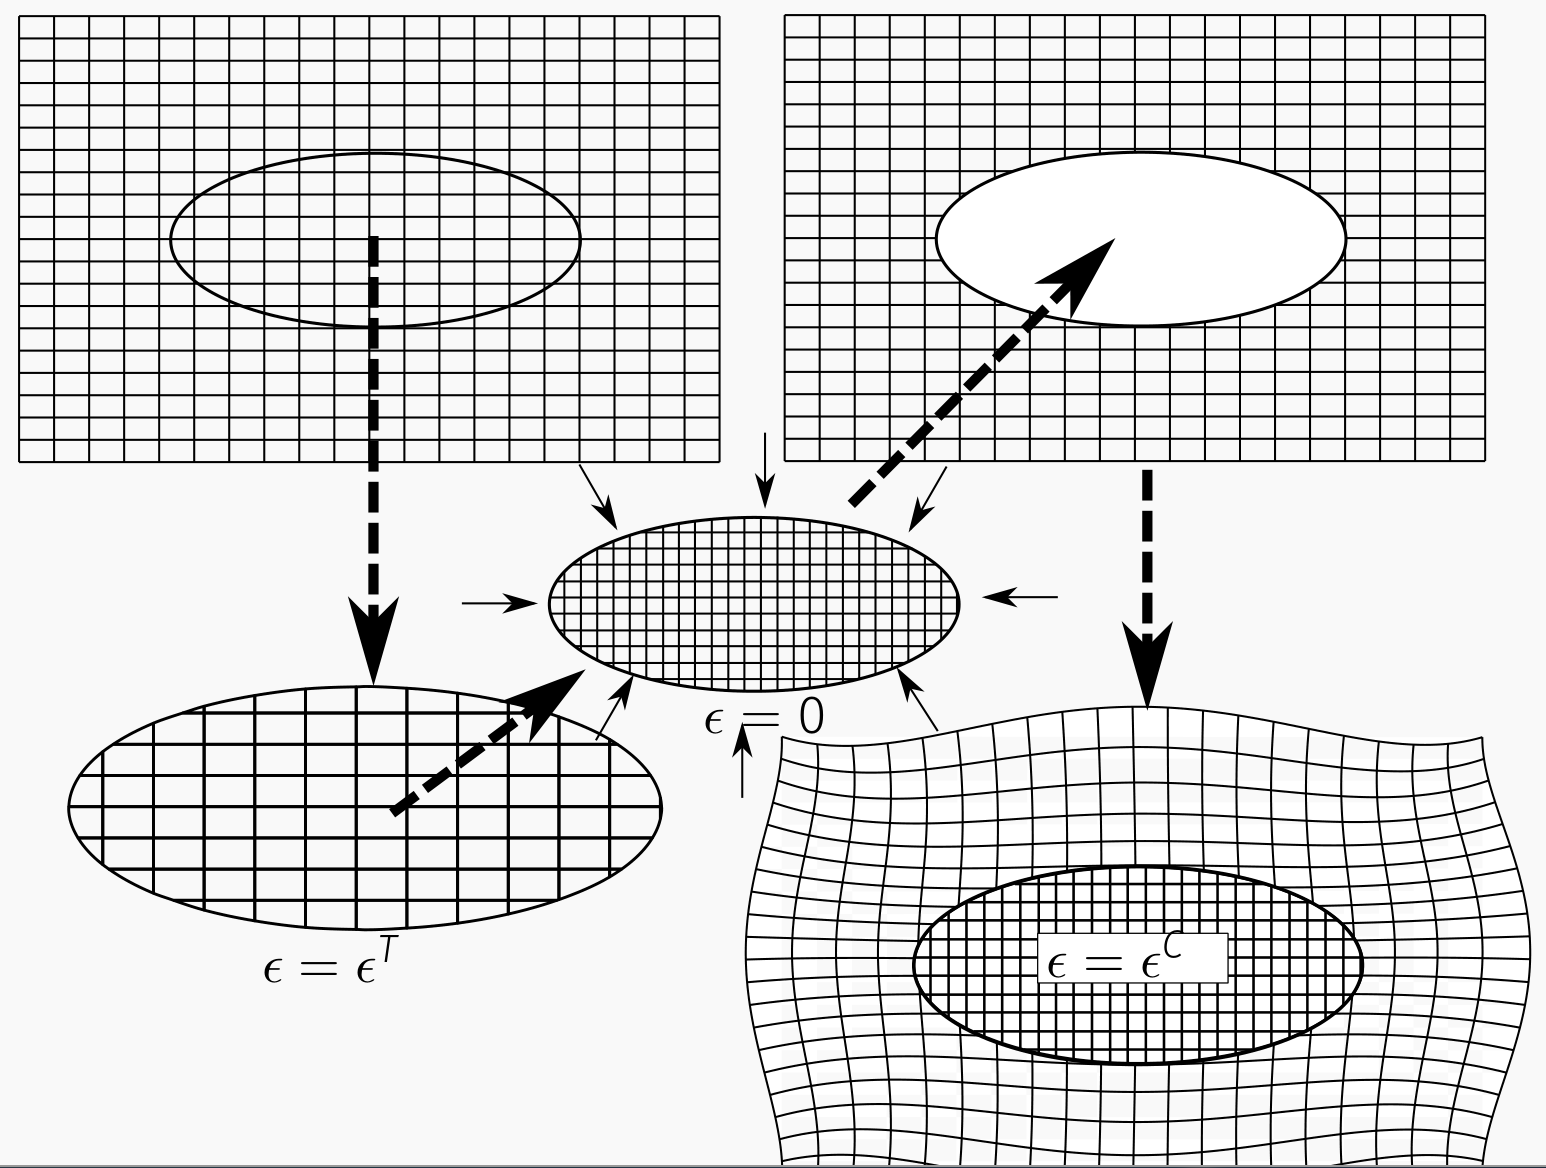
\includegraphics{../images/eshelby.png}
\end{frame}

\begin{frame}{eshelby's thought experiment}
\protect\hypertarget{eshelbys-thought-experiment-2}{}
\begin{itemize}
\tightlist
\item
  Now, we weld that expanded ellipsoid back into the original body
\item
  Tractions need to be applied to force it to fit
\item
  Once the stresses equilibrate, the ellipsoid has a constrained strain,
  \(\epsilon^C\)
\end{itemize}
\end{frame}

\begin{frame}{eshelby}
\protect\hypertarget{eshelby-1}{}
\begin{itemize}
\tightlist
\item
  After equilibrium is reached the inclusion is still under a state of
  uniform strain
\item
  The inclusion stress, \(\sigma_I\) can be found as:
\end{itemize}

\[\sigma_I = C_m (\epsilon^C - \epsilon^T)\]

Where \(C_m\) is the stiffness of the material.
\end{frame}

\begin{frame}{eshelby}
\protect\hypertarget{eshelby-2}{}
\begin{itemize}
\tightlist
\item
  One of Eshelby's critical findings is that
\end{itemize}

\[\epsilon^C = S \epsilon^T\]

\begin{itemize}
\tightlist
\item
  \emph{S} is known as the Eshelby Tensor, and is a fourth-order tensor
\item
  Function of shape and poisson's ratio
\item
  It has been calculated exactly for ellipsoids, and numerically for
  other shapes
\end{itemize}
\end{frame}

\begin{frame}{eshelby tensor}
\protect\hypertarget{eshelby-tensor}{}
\begin{itemize}
\tightlist
\item
  \(\nu\) represents the matrix Poisson's ratio
\item
  \emph{s} is the aspect ratio of the fibers
\item
  \(I_1 = \frac{2s}{\left(s^2-1\right)^{\frac{3}{2}}}(s{\left(s^2-1\right)}^{\frac{1}{2}}-\cosh^{-1} s)\)
\item
  \(Q=\frac{3}{8(1-\nu)}\)
\item
  \(R=\frac{1-2\nu}{8(1-\nu)}\)
\item
  \(T=\frac{Q\left(4-3I_1\right)}{3(s^2-1)}\)
\item
  \(I_3 = 4-2I_1\)
\end{itemize}
\end{frame}

\begin{frame}{eshelby tensor}
\protect\hypertarget{eshelby-tensor-1}{}
\begin{longtable}[]{@{}
  >{\centering\arraybackslash}p{(\columnwidth - 4\tabcolsep) * \real{0.24}}
  >{\centering\arraybackslash}p{(\columnwidth - 4\tabcolsep) * \real{0.68}}
  >{\centering\arraybackslash}p{(\columnwidth - 4\tabcolsep) * \real{0.08}}@{}}
\toprule
\(S_{ijkl}\) & Long Fibers & Short Fibers (Ellipsoids) \\
\midrule
\endhead
\(S_{1111}=S_{2222}\) & \(\frac{5-\nu}{8(1-\nu)}\) &
\(Q+RI_1+\frac{3T}{4}\) \\
\(S_{3333}\) & 0 & \(\frac{4Q}{3}+RI_3+2s^2T\) \\
\(S_{1122} = S_{2211}\) & \(\frac{-1+4\nu}{8(1-\nu)}\) &
\(\frac{Q}{3}-RI_1+\frac{4T}{3}\) \\
\(S_{1133} = S_{2233}\) & \(\frac{\nu}{2(1-\nu)}\) &
\(-R I_1 - s^2T\) \\
\(S_{3311} = S_{3322}\) & 0 & \(-R I_3 - T\) \\
\(\begin{aligned} S_{1212} & = S_{1221} \\& = S_{2112}=S_{2121} \end{aligned}\)
& \(\frac{3-4\nu}{8\left(1-\nu\right)}\) &
\(\frac{Q}{3}+RI_1+\frac{T}{4}\) \\
\(\begin{aligned} S_{1313} & = S_{1331} \\&=S_{3113}=S_{3131}\\&=S_{3232}=S_{3223}\\&=S_{2332}=S_{2323} \end{aligned}\)
& \(\frac{1}{4}\) & \(2R-\frac{I_1R}{2}-\frac{1+s^2}{2}T\) \\
all other \(S_{ijkl}\) & 0 & 0 \\
\bottomrule
\end{longtable}
\end{frame}

\begin{frame}{inclusions}
\protect\hypertarget{inclusions}{}
\begin{itemize}
\tightlist
\item
  Eshelby's initial thought experiment was for a homogeneous material
\item
  To consider a different type of inclusion, we need to relate the
  transformation strain between some fictitious ellipsoid of matrix
  material which would be equivalent to our inclusion.
\item
  We will refer to the inclusion stiffness as \(C_f\), the
  transformation strain in the matrix as \(\epsilon^T\), and the
  transformation strain in the inclusion \(\epsilon^{T*}\).
\end{itemize}
\end{frame}

\begin{frame}{inclusions}
\protect\hypertarget{inclusions-1}{}
\begin{itemize}
\tightlist
\item
  We are trying to find a transformation equivalent to our inclusion, so
  we set
\end{itemize}

\[\sigma_I = C_m(\epsilon^C - \epsilon^T) = C_f(\epsilon^C-\epsilon^{T*})\]

\begin{itemize}
\tightlist
\item
  Now we substitute the relation \(\epsilon^C = S\epsilon^T\)
\end{itemize}

\[C_m(S - I)\epsilon^T = C_f(S \epsilon^T-\epsilon^{T*})\]
\end{frame}

\begin{frame}{inclusions}
\protect\hypertarget{inclusions-2}{}
\begin{itemize}
\tightlist
\item
  We can solve this to find the transformation strain
\end{itemize}

\[\epsilon^T = \left [ (C_f - C_m)S + C_m\right]^{-1} C_f \epsilon^{T*}\]

\begin{itemize}
\tightlist
\item
  Since the transformation strain is arbitrary, we can choose
  \(\epsilon^T\) such that \(\epsilon^{T*}\) is 0
\item
  Now suppose we impose some strain, \(\epsilon^0\) on the composite
\end{itemize}
\end{frame}

\begin{frame}{stiffness}
\protect\hypertarget{stiffness}{}
\begin{itemize}
\tightlist
\item
  The stress in the inclusion will be
\end{itemize}

\[\sigma_I = C_m (\epsilon^0 + \epsilon^C - \epsilon^T) = C_f (\epsilon^0 + \epsilon^C)\]

\begin{itemize}
\tightlist
\item
  Simplifying terms gives
\end{itemize}

\[\left ( C_f - C_m \right ) \left ( \epsilon^0 + \epsilon^C \right) = -C_m \epsilon^T\]
\end{frame}

\begin{frame}{stiffness}
\protect\hypertarget{stiffness-1}{}
\begin{itemize}
\tightlist
\item
  We now assume \(\epsilon^0 + \epsilon^C = \bar{\epsilon}^f\) and
  multiply both sides by \(S C_m^{-1}\)
\end{itemize}

\[S \left( C_m \right ) ^{-1} \left ( C_f - C_m \right ) \bar{\epsilon}^f = -\epsilon^C\]

\begin{itemize}
\tightlist
\item
  Recall \(S\epsilon^T = \epsilon^C\)
\item
  We can also write \(\epsilon^C\) in terms of \(\bar{\epsilon}^f\)
\end{itemize}

\[S \left( C_m \right ) ^{-1} \left ( C_f - C_m \right ) \bar{\epsilon}^f = \epsilon^0- \bar{\epsilon}^f\]
\end{frame}

\begin{frame}{strain concentration}
\protect\hypertarget{strain-concentration}{}
\begin{itemize}
\tightlist
\item
  Finally, we can add \(I\bar{\epsilon}^f\) to both sides to find
\end{itemize}

\[[I+S \left( C_m \right ) ^{-1} \left ( C_f - C_m \right )] \bar{\epsilon}^f = \epsilon^0\]

\begin{itemize}
\tightlist
\item
  We define the inverse of the left-hand side the Eshelby
  strain-concentration tensor
\end{itemize}

\[A^E = [I+S \left( C_m \right ) ^{-1} \left ( C_f - C_m \right )]^{-1}\]

\begin{itemize}
\tightlist
\item
  The stiffness can be calculated as
\end{itemize}

\[C = C_m + v_i (C_f-C_m)A^E\]
\end{frame}

\begin{frame}{stiffness}
\protect\hypertarget{stiffness-2}{}
\begin{itemize}
\tightlist
\item
  This stiffness calculation is valid for any number of inclusions
\item
  However, it is only appropriate for very dilute concentrations
  (\textless1\% volume fraction)
\item
  This ensures that the assumption
  \(\epsilon^0 + \epsilon^C = \bar{\epsilon}^f\)
\end{itemize}
\end{frame}

\hypertarget{aspect-ratio}{%
\section{aspect ratio}\label{aspect-ratio}}

\begin{frame}{aspect ratio}
\protect\hypertarget{aspect-ratio-1}{}
\begin{itemize}
\tightlist
\item
  Some studies have been done to evaluate Eshelby tensors for short
  fibers
\item
  Long fibers are approximated by an ellipsoid with infinitely long
  major axis
\item
  This is not appropriate for short fibers
\item
  We could logically consider three different ellipsoids to represent a
  short fiber
\end{itemize}
\end{frame}

\begin{frame}{aspect ratio}
\protect\hypertarget{aspect-ratio-2}{}
\begin{figure}
\centering
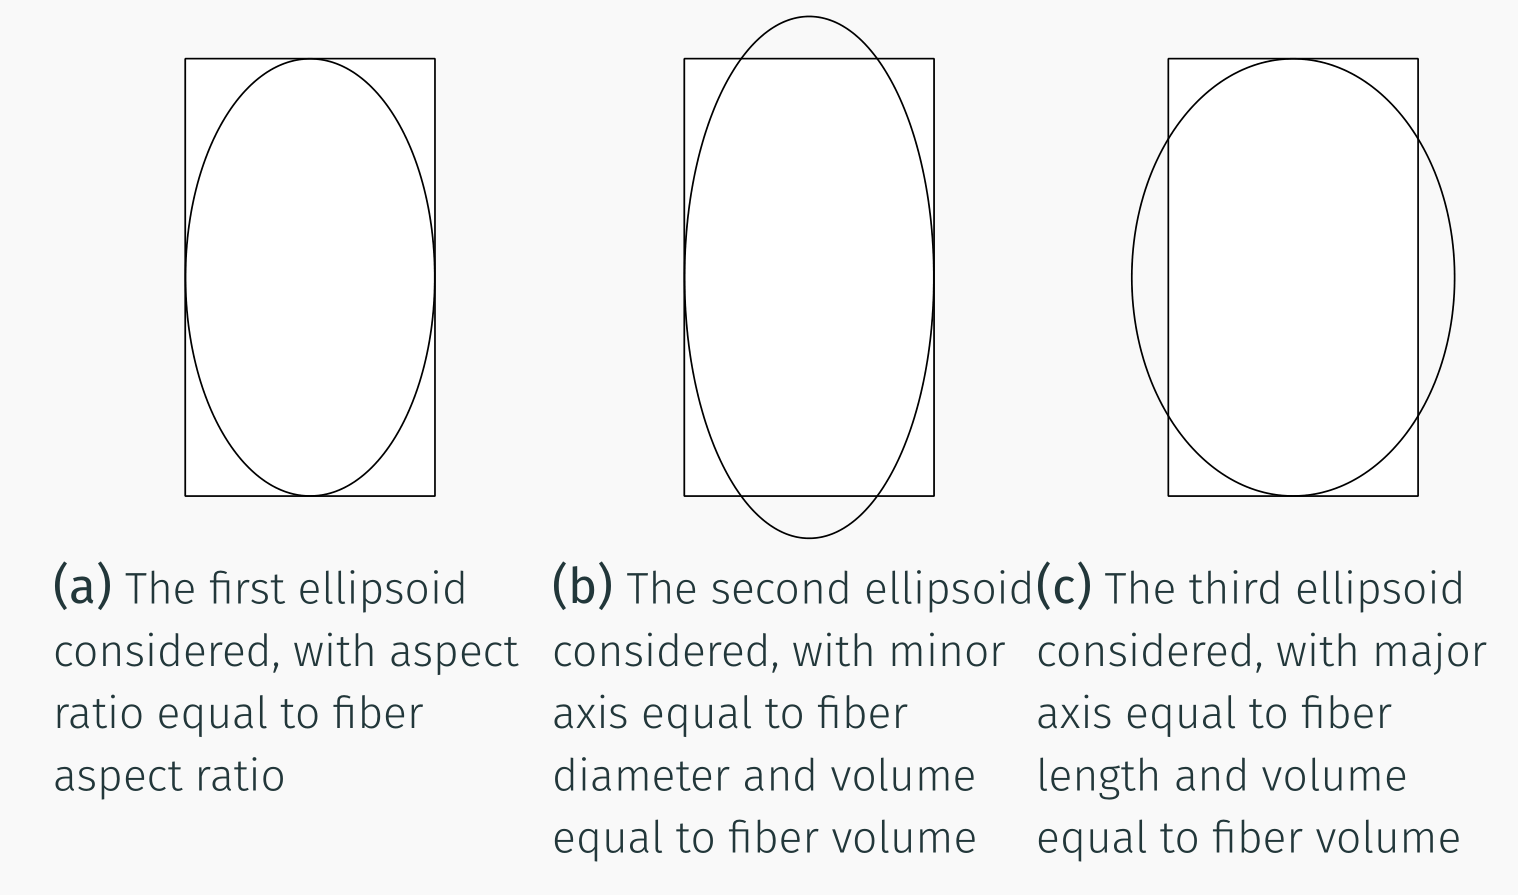
\includegraphics{../images/ellipsoids.PNG}
\caption{aspect ratio comparisons}
\end{figure}
\end{frame}

\begin{frame}{aspect ratio}
\protect\hypertarget{aspect-ratio-3}{}
\begin{itemize}
\item
  Steif and Hoysan investigated the effect of aspect ratio numerically
\item
  Found that (a) and (c) were good for short fibers
\item
  As fibers get longer, and as stiffness ratio of fiber to matrix
  increases, (a) gives best results
\item
  \begin{enumerate}
  [(a)]
  \tightlist
  \item
    is also the easiest to use (same aspect ratio), so that is what is
    done in Eshelby-based models
  \end{enumerate}
\end{itemize}
\end{frame}

\begin{frame}{fiber orientation}
\protect\hypertarget{fiber-orientation}{}
\begin{itemize}
\tightlist
\item
  With Eshelby (and derivative models), fibers at different orientations
  are modeled as a different inclusion
\item
  Since the Eshelby tensor, \emph{S} is a fourth-order tensor, we can
  treat it the same way as \emph{C}
\item
  Write it as 6x6 matrix, transform using \(R^\sigma\)
\end{itemize}
\end{frame}

\begin{frame}{example}
\protect\hypertarget{example}{}
\begin{itemize}
\tightlist
\item
  As an example, let us consider a ``laminate'' of short fiber
  composites
\item
  This is a good approximate for many 3D printed composites
\item
  We have a \(\pm 45^\circ\) laminate, with very short carbon fibers,
  \emph{s} = 15
\end{itemize}
\end{frame}

\begin{frame}{example}
\protect\hypertarget{example-1}{}
\begin{itemize}
\tightlist
\item
  First we find the Eshelby tensor for \emph{s} = 15
\item
  We also need the matrix Poisson's ratio, \(\nu = 0.4\)
\item
  We find the parameters \protect\hyperlink{ux2feshelby-params}{here}
\item
  Then we use \protect\hyperlink{ux2feshelby-table}{this slide} to find
  \(S_{ijkl}\)
\item
  Notice that this assumes fibers are pointed in the 3-direction
\end{itemize}
\end{frame}

\begin{frame}{example}
\protect\hypertarget{example-2}{}
\begin{itemize}
\tightlist
\item
  Next, we rotate \(S_{ijkl}\) to find \(S^{45}\) and \(S^{-45}\)
\item
  Notice: the eshelby tensor, \emph{S} accounts for rotation, we do not
  rotate \(C_f\)
\item
  So we find \(A^{45}\) and \(A^{-45}\)
\end{itemize}

\[A^{45} = \left[I + S^{45} (C_m)^{-1}(C_f-C_m) \right]^{-1}\]

\[A^{-45} = \left[I + S^{-45} (C_m)^{-1}(C_f-C_m) \right]^{-1}\]
\end{frame}

\begin{frame}{example}
\protect\hypertarget{example-3}{}
\begin{itemize}
\tightlist
\item
  This gives our total stiffness calculation as
\end{itemize}

\[C = C_m + v^{45}(C_f-C_m)A^{45} + v^{-45}(C_f-C_m)A^{-45}\]

\begin{itemize}
\tightlist
\item
  If we assume the volume fraction of fibers in our part is 20\%
\item
  And that there are equally many fibers in 45 and -45 directions
\item
  Then \(v^{45} = v^{-45} = 0.1\)
\item
  Note: Since this is not a dilute concentration, we would not expect
  this to be very accurate
\end{itemize}
\end{frame}

\begin{frame}{example}
\protect\hypertarget{example-4}{}
\begin{itemize}
\tightlist
\item
  Python code for this example (with some typical values for \(C_m\) and
  \(C_f\)) is posted
  \href{https://colab.research.google.com/drive/1aUs_BfeWugyUfwQiKoPx5g-hxvrsQqNs?usp=sharing}{here}
\end{itemize}
\end{frame}

\hypertarget{fiber-orientation-1}{%
\section{fiber orientation}\label{fiber-orientation-1}}

\begin{frame}{fiber orientation}
\protect\hypertarget{fiber-orientation-2}{}
\begin{itemize}
\tightlist
\item
  While a laminate analogy works well for some cases, in general short
  fibers are not aligned in laminates
\item
  It is not practical to model each possible fiber orientation as a
  separate inclusion
\item
  Advani-Tucker introduced a tensorial representation of fiber
  orientation
\end{itemize}
\end{frame}

\begin{frame}{fiber in spherical coordinates}
\protect\hypertarget{fiber-in-spherical-coordinates}{}
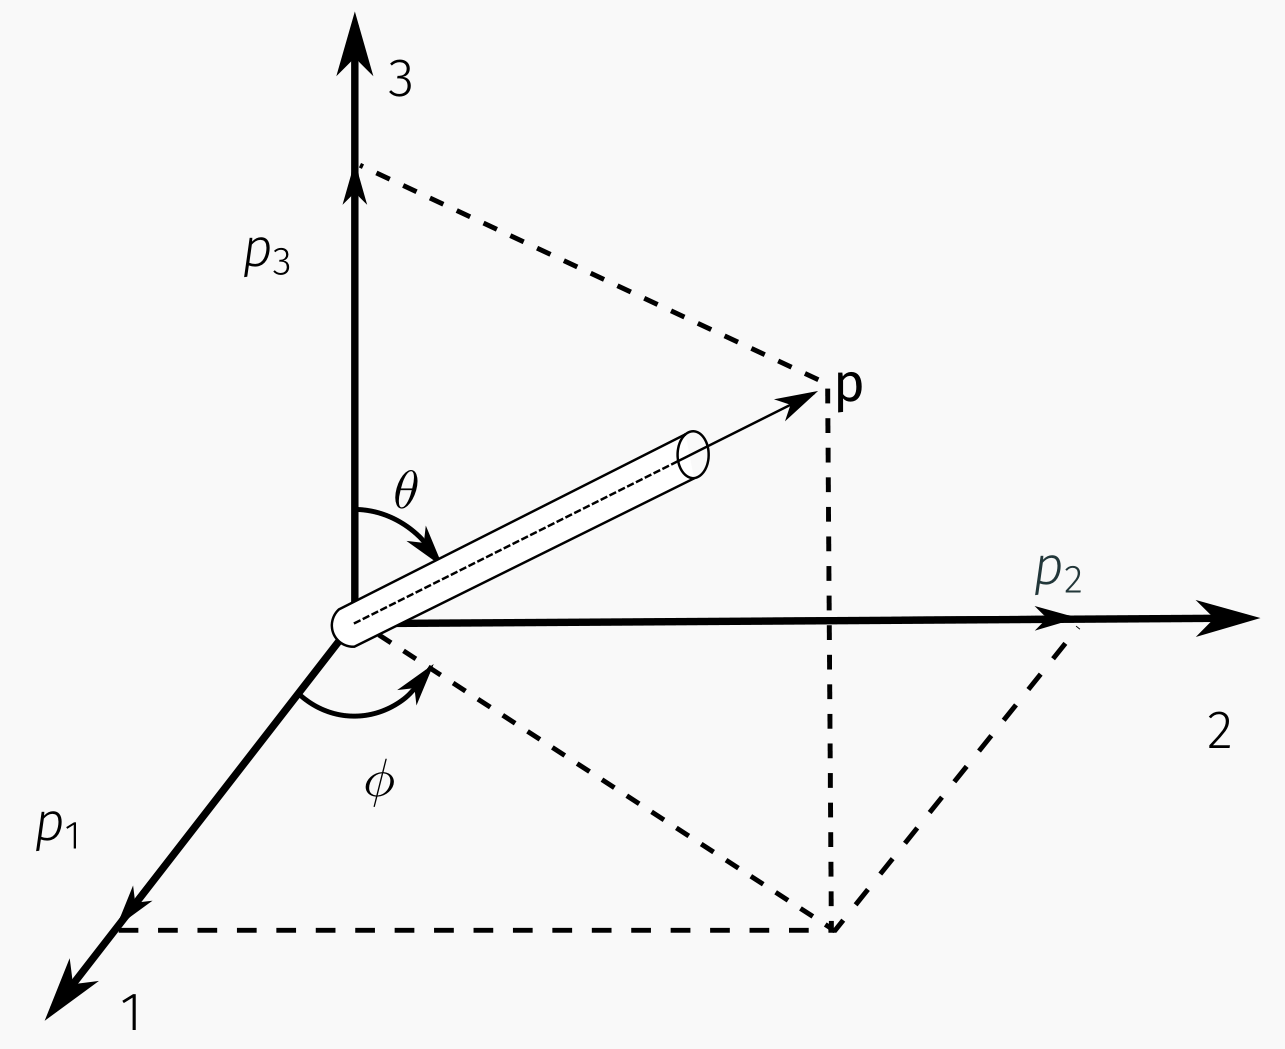
\includegraphics{../images/single_fiber.png}
\end{frame}

\begin{frame}{fiber direction components}
\protect\hypertarget{fiber-direction-components}{}
\begin{longtable}[]{@{}ll@{}}
\toprule
Component & Definition \\
\midrule
\endhead
\(p_1\) & \(\sin \theta \cos \phi\) \\
\(p_2\) & \(\sin \theta \sin \phi\) \\
\(p_3\) & \(\cos \theta\) \\
\bottomrule
\end{longtable}
\end{frame}

\begin{frame}{orientation tensor}
\protect\hypertarget{orientation-tensor}{}
\begin{itemize}
\tightlist
\item
  Within a given volume, a distribution of fibers can be defined by some
  orientation distribution function, \(\psi(\theta, \phi)\).
\item
  Advani and Tucker introduced tensor representations of fiber
  orientation distribution functions
\end{itemize}

\[a_{ij} = \oint p_i p_j \psi(p) dp\]
\end{frame}

\begin{frame}{orientation tensor}
\protect\hypertarget{orientation-tensor-1}{}
\begin{itemize}
\tightlist
\item
  And
\end{itemize}

\[a_{ijkl} = \oint p_i p_j p_k p_l\psi(p) dp\]

\begin{itemize}
\tightlist
\item
  Note: any order tensor may be defined in this manner, the orientation
  distribution function must be even, due to fiber symmetry, and thus
  any odd-ordered tensor will be zero.
\end{itemize}
\end{frame}

\begin{frame}{orientation tensor}
\protect\hypertarget{orientation-tensor-2}{}
\begin{itemize}
\tightlist
\item
  It can be noted that some symmetries must exist due to the way the
  tensors are defined.
\item
  In the second order tensor we have
\end{itemize}

\[a_{ij} = a_{ji}\]

\begin{itemize}
\tightlist
\item
  and in the fourth order tensor
\end{itemize}

\[a_{ijkl} = a_{jikl} = a_{kijl}\]

and so on for any permutation of i, j, k and l.
\end{frame}

\begin{frame}{orientation tensor}
\protect\hypertarget{orientation-tensor-3}{}
\begin{itemize}
\tightlist
\item
  The orientation tensor is also normalized such that:
\end{itemize}

\[a_{ii} = 1\]

\begin{itemize}
\tightlist
\item
  And any lower-order tensor can be expressed in terms of the next
  higher-order tensor, for example
\end{itemize}

\[a_{ijkk} = a_{ij}\]
\end{frame}

\begin{frame}{example - 2D random}
\protect\hypertarget{example---2d-random}{}
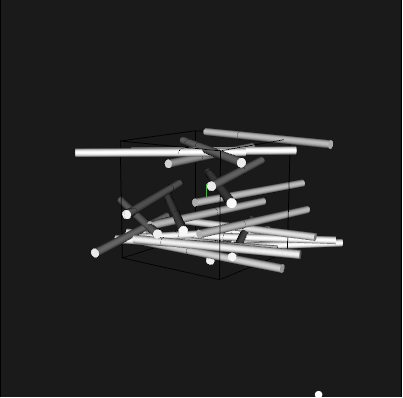
\includegraphics{../images/random2D.PNG}

A visualization of a 2D random orientation distribution. This is
expressed with the second-order tensor \(a_{11} = a_{22} = 0.5\) with
all other \(a_{ij} = 0\).
\end{frame}

\begin{frame}{example - 3D random}
\protect\hypertarget{example---3d-random}{}
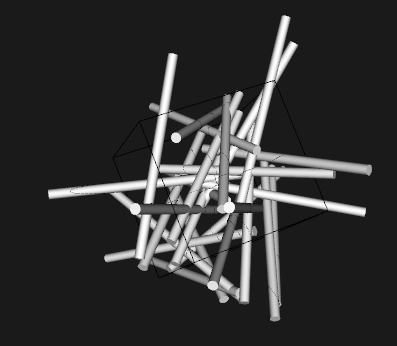
\includegraphics{../images/random3D.PNG}

A visualization of a 3D random orientation distribution. This is
expressed with the second-order tensor
\(a_{11} = a_{22} = a_{33} = 1/3\) with all other \(a_{ij} = 0\).
\end{frame}

\begin{frame}{example - aligned 45}
\protect\hypertarget{example---aligned-45}{}
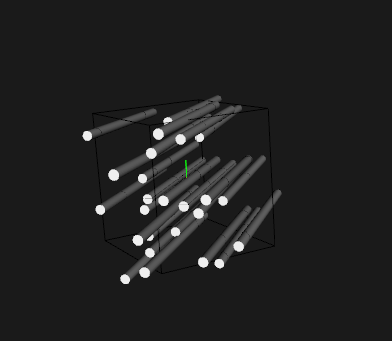
\includegraphics{../images/aligned45.PNG}

A visualization of a perfectly aligned, off-axis orientation
distribution. This is expressed by rotating the tensor with
\(a_{11} = 1\) and all other \(a_{ij} = 0\).
\end{frame}

\begin{frame}{next class}
\protect\hypertarget{next-class}{}
\begin{itemize}
\tightlist
\item
  Orientation averaging
\item
  Self-consistent and Mori-Tanaka methods
\end{itemize}
\end{frame}

\end{document}
